\section{Documentation for programmers}
\subsection{Specification}
The program implements a DHCP relay. Figure~\ref{fig:dhcp} depicts how it works.
\begin{figure}[h]
	\centering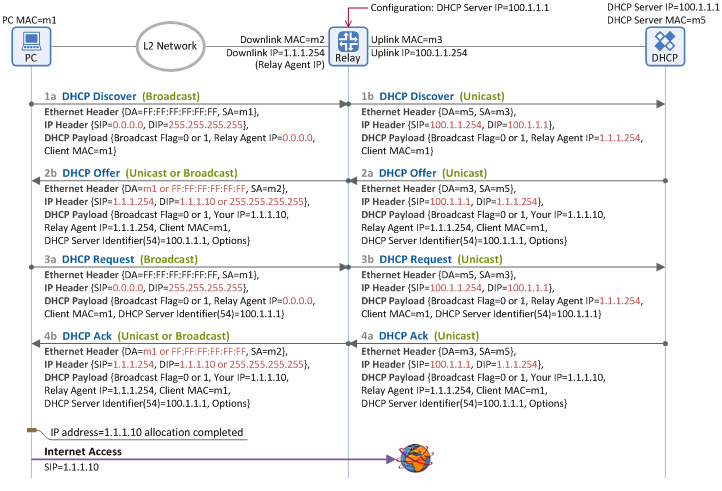
\includegraphics[scale=0.5]{images/dhcp}
	\caption{DHCP relay\protect\footnotemark}
	\label{fig:dhcp}
\end{figure}
\footnotetext{\url{https://www.netmanias.com/en/?m=view\&id=techdocs\&no=6000}}

Basically, a DHCP relay is a ``man in the middle'' between the client and the DHCP server. It helps the client to contact the server in order to obtain an IP address. It does so receiving the broadcast packets sent by clients and forwarding them in an unicast connection to one (or more) DHCP servers, and vice versa, forwarding the server responses in broadcast to the clients. 

While modeling its behavior, we refer to the above figure. We suppose to be able to detect when a message comes from a client and when it comes from a server by means of two different interruptions, without looking at the \texttt{OPCode} field (which is 1 for a request and 2 for a response). In other words, two \textit{different events} occur. This is reasonable, since Figure~\ref{fig:dhcp} depicts two different links (\textit{Downlink} and \textit{Uplink}), with two different MAC and IP addresses. 

Our ASG diagram is depicted in Figure~\ref{fig:asg}.

\begin{figure}[h]
	\centering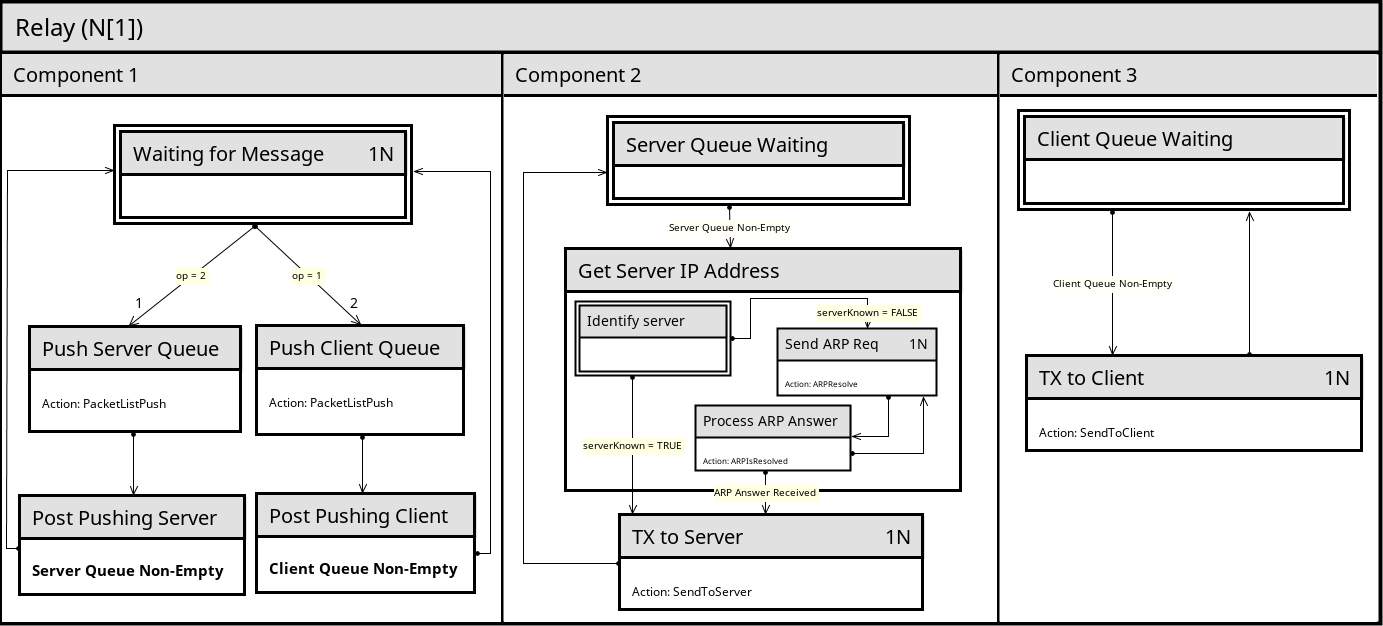
\includegraphics[scale=0.4]{images/asg-diagram}
	\caption{ASG diagram modeling a DHCP relay}
	\label{fig:asg}
\end{figure}

A DHCP relay consists of four parallel components following a producer-consumer pattern. Two components, 1 and 3, wait for a packet, either from a client (broadcast) or a server (unicast). They then modify this packet as follows:
\begin{itemize}
	\item \textbf{Component 1} - \texttt{ModifyServerPacket}:
	\begin{itemize}
		\item \textbf{Ethernet Payload}
		\begin{itemize}
			\item Destination MAC Address: DHCP Relay Uplink MAC $\to$ Broadcast
			\item Source MAC Address: DHCP Server MAC $\to$ DHCP Relay MAC Address
		\end{itemize} 
			\item \textbf{IP Payload}
		\begin{itemize}
			\item Source IP Address: DHCP Server IP Address $\to$ DHCP Relay Downlink IP
			\item Destination IP Address: DHCP Relay Downlink IP $\to$ Broadcast
		\end{itemize}	
	\end{itemize}
	\item \textbf{Component 2} - \texttt{ModifyClientPacket}:
	\begin{itemize}
		\item \textbf{Ethernet Payload}
		\begin{itemize}
			\item Destination MAC Address: Broadcast $\to$ DHCP Server MAC
			\item Source MAC Address: PC MAC Address $\to$ DHCP Relay Uplink MAC 
		\end{itemize}
		\item \textbf{IP Payload}
		\begin{itemize}
			\item Source IP Address: 0.0.0.0 (no IP address) $\to$ DHCP Relay Uplink IP
			\item Destination IP Address: Broadcast $\to$ DHCP Server IP
		\end{itemize}
		\item \textbf{DHCP Payload}
		\begin{itemize}
			\item Gateway IP Address (GIADDR): 0.0.0.0 $\to$ DHCP Relay Downlink IP
		\end{itemize}
	\end{itemize}
\end{itemize}

The two components then push the modified packet in a queue (two different queues are present, respectively for server and client) and set a rendez-vous (respectively \textbf{Client New Message} and \textbf{Server New Message}) to awake the corresponding consumer.

Component 2 and 4 represent the consumers. If they are waiting, they are awoke by a push of the corresponding producer. Once a message is received, they enter the transmission state, and leave it only when the queue is empty. Here they continuously pop an element from the queue and send it in broadcast (Component 2) or in unicast to one (or more) DHCP servers (Component 4).

This separation in two producers-consumers allow us to separate two logical different operations: handling the traffic incoming client-side and the one incoming server-side. 